\chapter{Data and Probability – Understanding Uncertainty and Making Predictions}

\section{Introduction: Why Data and Probability Matter}
Data is everywhere. Whether it's tracking your daily steps, measuring the weather, or evaluating trends in social media, we rely on data to help us make sense of the world. Data helps us understand patterns, make predictions, and make informed decisions.

Probability, on the other hand, is the branch of math that deals with uncertainty. It helps us understand how likely something is to happen. From deciding whether to bring an umbrella based on the chance of rain, to predicting the outcome of a game, probability plays an essential role in our decision-making process.

In this chapter, we'll dive into the basics of data and probability, exploring how to interpret and use data, and how to calculate the likelihood of different events.

\section{What Is Data?}
Data refers to facts, figures, or information that can be measured and analyzed. Data comes in two main types:

\begin{itemize}
    \item \textbf{Qualitative Data:} Data that describes characteristics or categories. For example, eye color (blue, brown, green) or favorite foods (pizza, pasta, sushi).
    \item \textbf{Quantitative Data:} Data that involves numbers. For example, the number of people in a classroom, the height of a tree, or the temperature outside.
\end{itemize}

We collect and analyze data to uncover patterns, identify trends, and make decisions.

\subsection{Organizing Data}
Data is often organized into tables, graphs, and charts to make it easier to understand.

\textbf{Example:} Imagine you're collecting data on how many books your classmates read in a month. Your data might look like this:

\begin{tabular}{|c|c|}
\hline
Name & Books Read \\
\hline
Sarah & 4 \\
John & 3 \\
Maria & 5 \\
David & 2 \\
\hline
\end{tabular}

From this table, you can easily see how many books each person read and compare the results.

\section{Using Graphs to Represent Data}
Graphs are visual representations of data, making it easier to see patterns and trends. Let’s explore a few common types of graphs:

\subsection{Bar Graph}
Used to compare quantities across different categories. Each bar represents a category, and the height or length of the bar shows the value.

\textbf{Example:} A bar graph showing the number of books read by your classmates:
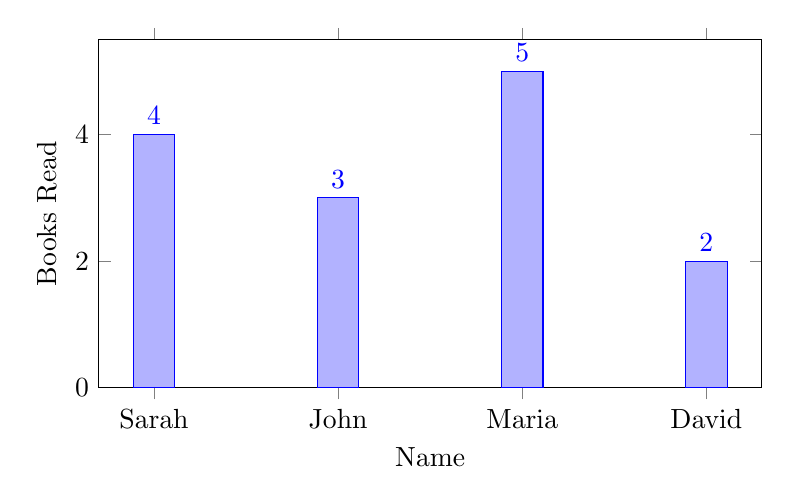
\begin{tikzpicture}
    \begin{axis}[
        ybar,
        symbolic x coords={Sarah, John, Maria, David},
        xtick=data,
        nodes near coords,
        ymin=0,
        ylabel={Books Read},
        xlabel={Name},
        bar width=15pt,
        width=10cm,
        height=6cm
    ]
    \addplot coordinates {(Sarah,4) (John,3) (Maria,5) (David,2)};
    \end{axis}
\end{tikzpicture}
\subsection{Line Graph}
Used to show changes over time. A line connects data points to show how something increases or decreases.

\textbf{Example:} If you track the temperature throughout a month, a line graph could show the daily changes in temperature.
\textbf{Example:} A line graph showing temperature changes over a 30-day period in Fahrenheit:
\begin{center}
    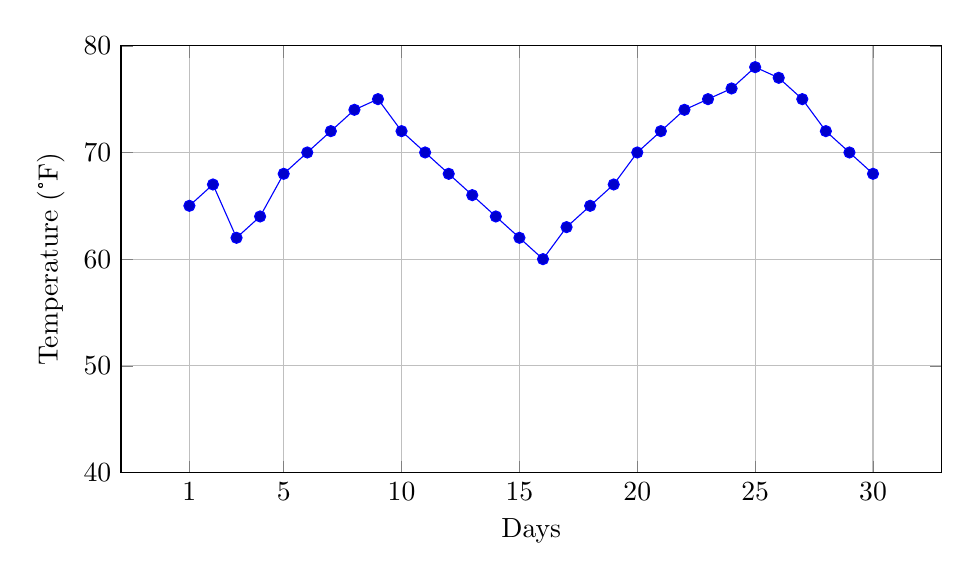
\begin{tikzpicture}
        \begin{axis}[
            xlabel={Days},
            ylabel={Temperature (°F)},
            xtick={1,5,10,15,20,25,30},
            ymin=40,
            ymax=80,
            grid=major,
            width=12cm,
            height=7cm
        ]
        \addplot coordinates {(1,65) (2,67) (3,62) (4,64) (5,68) (6,70) (7,72) 
        (8,74) (9,75) (10,72) (11,70) (12,68) (13,66) (14,64) 
        (15,62) (16,60) (17,63) (18,65) (19,67) (20,70) 
        (21,72) (22,74) (23,75) (24,76) (25,78) (26,77) 
        (27,75) (28,72) (29,70) (30,68)};
        \end{axis}
    \end{tikzpicture}
\end{center}

\subsection{Pie Chart}
Used to show parts of a whole. Each "slice" of the pie represents a percentage of the total.

\textbf{Example:} A pie chart could show the percentage of time you spend on different activities in a day, like studying, exercising, and sleeping.

\section{What Is Probability?}
Probability is the study of how likely something is to happen. It’s a way of measuring uncertainty. The probability of an event can range from 0 to 1:

\begin{itemize}
    \item A probability of 0 means the event is impossible (it will never happen).
    \item A probability of 1 means the event is certain (it will definitely happen).
    \item Any probability between 0 and 1 reflects varying levels of likelihood.
\end{itemize}

\textbf{Example:}

If you're flipping a coin, there are two possible outcomes: heads or tails. Since the coin is fair, each outcome has an equal probability of happening:

\begin{itemize}
    \item The probability of getting heads is $\frac{1}{2}$ or 0.5.
    \item The probability of getting tails is also $\frac{1}{2}$ or 0.5.
\end{itemize}

\section{Calculating Probability}
The basic formula for probability is:

\[
\text{Probability of an event} = \frac{\text{Number of favorable outcomes}}{\text{Total number of possible outcomes}}
\]

\textbf{Example 1: Rolling a Die}

If you roll a standard six-sided die, the probability of rolling a 4 is:

\begin{itemize}
    \item Favorable outcome: 1 (only one side of the die has a 4).
    \item Total possible outcomes: 6 (since the die has six sides).
\end{itemize}

\[
\text{Probability of rolling a 4} = \frac{1}{6}
\]

\textbf{Example 2: Drawing a Card}

If you draw one card from a standard deck of 52 cards, the probability of drawing a heart is:

\begin{itemize}
    \item Favorable outcomes: 13 (since there are 13 hearts in a deck).
    \item Total possible outcomes: 52.
\end{itemize}

\[
\text{Probability of drawing a heart} = \frac{13}{52} = \frac{1}{4}
\]

\section{Complementary and Independent Events}
\subsection{Complementary Events}
Complementary events are two events where one must happen, and the other cannot. For example, when flipping a coin, you either get heads or tails, but not both. The probability of the two events adds up to 1.

If the probability of an event is $P$, then the probability of its complement (the event not happening) is:

\[
\text{Probability of complement} = 1 - P
\]

\textbf{Example:}

If the probability of rain tomorrow is 0.3, the probability that it will not rain is:

\[
1 - 0.3 = 0.7 \text{ or } 70\%
\]

\subsection{Independent Events}
Independent events are events where the outcome of one does not affect the outcome of the other. For example, rolling a die and flipping a coin are independent events because the result of the die does not impact the coin flip.

For independent events, the probability of both events happening is the product of their individual probabilities.

\textbf{Example:}

If the probability of rolling a 6 on a die is $\frac{1}{6}$, and the probability of flipping heads on a coin is $\frac{1}{2}$, the probability of both rolling a 6 and flipping heads is:

\[
\text{Probability of both} = \frac{1}{6} \times \frac{1}{2} = \frac{1}{12}
\]

\section{Making Predictions with Probability}
Probability helps us make predictions about future events based on past data or known probabilities.

\textbf{Example:}

If you know that the chance of rain tomorrow is 60\%, you might decide to bring an umbrella because the probability suggests that it’s more likely to rain than not.

In sports, teams use probability to predict the chances of winning based on previous games, player performance, and conditions like weather or location.

\section{Understanding Averages (Mean, Median, and Mode)}
When analyzing data, it’s often useful to find a measure of central tendency—a number that represents the "middle" or typical value in a set of data. The three most common measures are mean, median, and mode.

\subsection{Mean (Average)}
Add up all the numbers and divide by how many numbers there are.

\textbf{Example:} The mean of 2, 4, 6, and 8 is:

\[
\frac{2 + 4 + 6 + 8}{4} = \frac{20}{4} = 5
\]

\subsection{Median}
The middle number in a sorted list.

\textbf{Example:} The median of 1, 3, and 5 is 3 (because 3 is in the middle).

\subsection{Mode}
The number that appears most often.

\textbf{Example:} In the set 2, 2, 3, 4, 4, 4, the mode is 4 (because it appears three times).

\section{Practice Makes Perfect: Let’s Try Some Exercises!}
\subsection{Probability}
\begin{itemize}
    \item What is the probability of rolling an even number on a six-sided die?
    \item If you flip a coin twice, what is the probability of getting heads both times?
\end{itemize}

\subsection{Data Interpretation}
\begin{itemize}
    \item A class survey found the following number of pets per student: 1, 2, 2, 3, 4, 4, 4, 5. Find the mean, median, and mode of this data.
    \item Draw a bar graph to represent the following data about how many people like different fruits:
    \begin{itemize}
        \item Apples: 10
        \item Bananas: 7
        \item Oranges: 5
    \end{itemize}
\end{itemize}

\section{Real-Life Applications of Data and Probability}
\begin{itemize}
    \item \textbf{Weather Forecasting:} Meteorologists use past data and probability to predict the likelihood of different weather conditions.
    \item \textbf{Health:} Doctors use probability to understand the chances of developing certain conditions based on risk factors like age, genetics, and lifestyle.
    \item \textbf{Games of Chance:} When playing games like dice, cards, or lotteries, probability helps determine the chances of winning.
\end{itemize}

\section{Chapter Summary}
\begin{itemize}
    \item Data helps us collect, organize, and analyze information to understand patterns and make decisions.
    \item Graphs like bar graphs, line graphs, and pie charts help us visualize data.
    \item Probability is the study of uncertainty and helps us measure how likely an event is to happen.
    \item We can calculate the probability of events using the formula: 
    
    \[
    \text{Probability} = \frac{\text{Number of favorable outcomes}}{\text{Total number of possible outcomes}}
    \]
    
    \item Complementary events are those where one event happens, and the other does not, with their probabilities adding up to 1.
    \item Independent events do not affect each other, and the probability of both occurring is the product of their individual probabilities.
    \item Mean, median, and mode are useful measures of central tendency that help summarize data.
\end{itemize}

\textbf{Challenge Question:}

You roll a six-sided die and flip a coin. What is the probability that you will roll a 4 and flip heads? Explain your reasoning.